\section{Pembagian bab}
Secara default pembagian bab pada latex menggunakan perintah \textit{section}, \textit{subsection}, \textit{subsubsection} dan \textit{subsubsubsection}. Untuk mengatur kedalaman suatu dokumen pada bab bab tertentu, kita dapat menggunakan perintah berikut ini pada bagian Preamble :
setcounter.secnumdepth
setcounter.tocdepth



Opsi yang digunakan pada syntax secnumdepth pada perintah verbcounter= seperti perintah diatas, berarti Anda telah merubah kedalaman bab yang Anda perbaharui sampai dengan level 5 yaitu section -- subsection -- subsubsection -- paragraph -- subparagraph. Sedangkan pada perintah dari opsi tocdepth berfungsi untuk membuat table of contents atau menampilkan kedalaman bab sampai dengan level 5, namun jika tidak di setel maka pada bagian level 3 kebawah tidak akan dapat ditampilkan pada bagian toc \ref{labelgambar}.


\begin{figure}[ht]
\centerline{\includegraphics[width=1\textwidth]{figures/capture.JPG}}
\caption{Pembagian Bab.}
\label{labelgambar}
\end{figure}


\section{Format Cetak}
Pada format LateX teks mempunyai bentuk plaintext, yang artinya teks tersebut belum diformat. Pada proses formatting teks dapat dilakukan dengan bahasa tersendiri yaitu bahasa markup. Hal paling mendasar antara lain cetak tebal, miring dan gari bawah. Cetak tebal menggunakan perintah \textit{textbf},cetak miring menggunakan perintah \textit{textit} dan garis bawah menggunakan perintah \textit{underline}.

\section{Tanda petik}
Tanda petik di Latex menggunakan petik miring dan petik satu. Petik miring biasanya berada pada sebelah angka satu di keyboard dan diakhiri petik satu. Ingat fungsi tanda petik hanya untuk melakukan quote atau pengutipan langsung. Untuk istilah bahasa inggris gunakan miring atau italic.

\begin{lstlisting}[caption=Contoh kalimat dalam tanda petik pada Latex,label={lst:tandapetik}]
`kalimat dalam tanda petik'
\end{lstlisting}


\section{Kode Program}
Agar kita dapat memasukan kode program, kita dapat menggunakan perintah \textit{lstlisting}. Perintah ini  berfungsi untuk memasukkan atau menambahkan kode program apapun ke dalam file yang terpisah. Untuk memasukan perintah \textit{lstlisting} kita perlu menulis parameter \textit{caption} dan \textit{label} untuk memberikan penjelasan keterangan kode program dan sebagai sumber referensi dari label kode program.

\lstinputlisting[caption=Menambahkan kode program,label={lst:kodeprogram}]{src/1/lstlisting.tex}


\section{Menambahkan Spesial Karakter}
Untuk menambahkan karakter spesial pada LaTex kita dapat menggunakan tanda \textit{backslash} didepan karakter yang ingin kita tandai. Terdapat beberapa karakter yang tidak bisa langsung digunakan seperti tanda \textit{ampersand}. Selain itu format pemberian kutipan pada LaTex berbeda dengan pemberian kutipan pada editor lainnya, cara memasukkan karakter spesial menggunakan listing \ref{lst:kodespesial}
\lstinputlisting[caption=Contoh kode untuk menambahkan karakter spesial,label={lst:kodespesial}]{src/1/spesial.tex}

\section{Menambahkan Chapter}
Berikut ini merupakan langkah-langkah untuk menambahkan \textit{chapter} baru.
\begin{enumerate}
\item Pertama kita buat \textit{chapter} baru pada repositori kita di folder \verb|chapters|, seperti pada gambar \ref{fig:tambahchapter}.

\begin{figure}[!htbp]
  \centering
  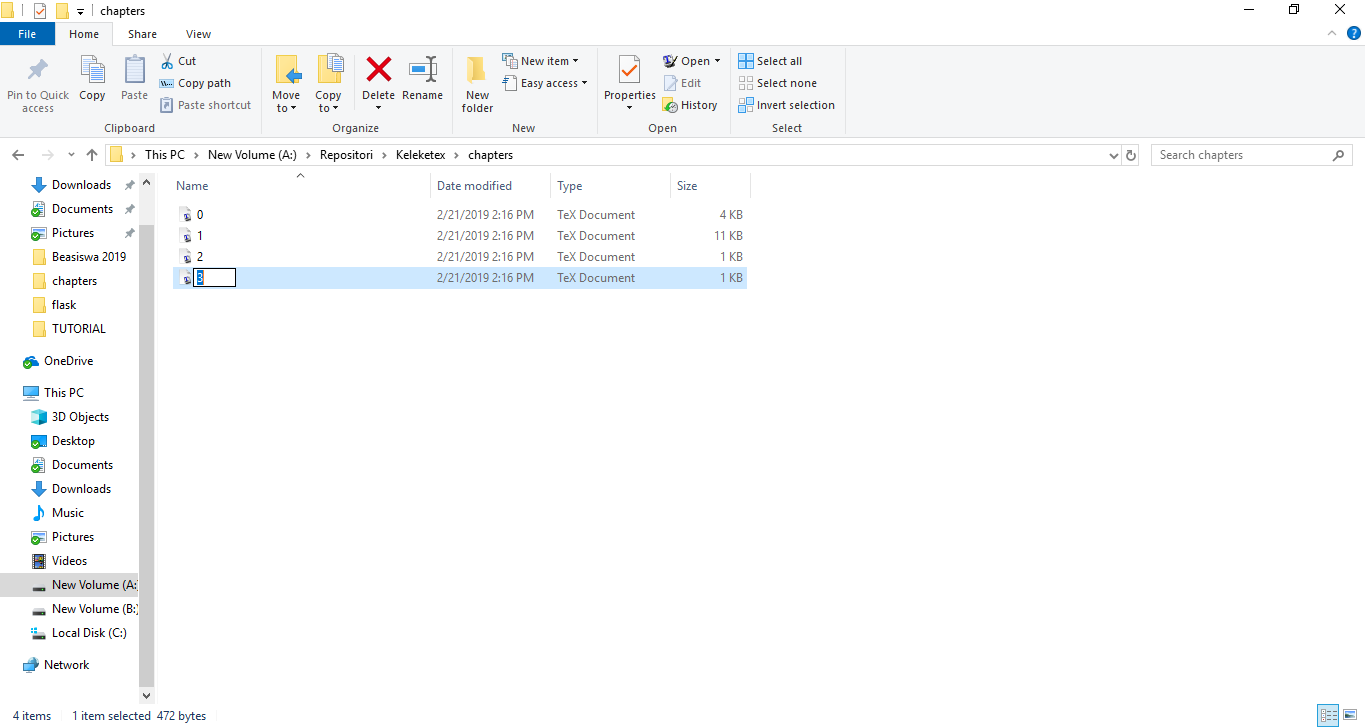
\includegraphics[width=.75\textwidth]{figures/tambahchapter.png}
  \caption{Menambahkan Chapter Baru}\label{fig:tambahchapter}
\end{figure}

\item Kemudian kita tambahkan kode seperti pada \textit{listing} \ref{lst:input} yang berfungsi untuk memanggil \textit{chapter} yang baru kita tambahkan pada file \verb|main.tex| seperti pada gambar \ref{fig:inputchapter}.

\lstinputlisting[caption=Penggunaan perintah input untuk menambahkan chapter,label={lst:input}]{src/1/input.tex}

\begin{figure}[!htbp]
  \centering
  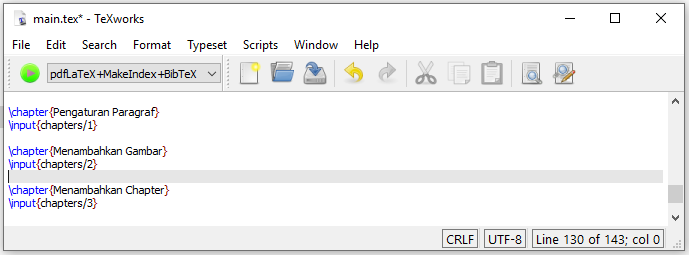
\includegraphics[width=.75\textwidth]{figures/inputchapter.png}
  \caption{Menambahkan Perintah Input Chapter}\label{fig:inputchapter}
\end{figure}

\item Terakhir, compile file \verb|main.tex| untuk melihat chapter baru yang telah kita tambahkan pada file main.pdf.
\end{enumerate}

\section{Perintah Include dan Input}
Ketika kita mengerjakan dokumen-dokumen besar menggunakan latex, tentunya kita akan memecah file menjadi beberapa bagian atau chapters agar isi dari dokumen tersebut lebih terorganisir atau terstruktur. Untuk itu latex memiliki 2 perintah untuk membantu kita semua agar dapat melakukan hal ini. Perintah tersebut tidak lain adalah perintah \textbf{include} dan \textbf{input}.
\subsection{Include} 
Perintah \textbf{include} bisa kita gunakan pada batang tubuh dokumen dan pada bagian main.tex, untuk menyisipkan isi file yang lain. Perintah include bisa digunakan untuk menyisipkan file chapter pada main.tex, gambar, link dan sebagainya. Pada gambar misalnya, biasanya akan ditambahkan perintah \textit{includegraphics} atau pada main.tex kita hanya perlu menambahkan perintah \textbf{include} pada chapter atau bagian yang ingin kita sisipkan. Hal yang perlu kita ketahui adalah latex akan memulai halaman baru sebelum memproses isi dari \textit{namafile}. Contoh penggunaan perintah \textit{includegraphics} dapat kita lihat pada gambar \ref{fig:inputchapter} dengan kode pemograman yang dilakukan seperti pada listing \ref{lst:graphic}

\lstinputlisting[caption=Penggunaan perintah includegraphics,label={lst:graphic}]{src/1/graphic.tex}

Dan berikut adalah contoh penggunaan perintah \textbf{include} pada main.tex dapat kita lihat dengan listing \ref{lst:include}

\lstinputlisting[caption=Penggunaan perintah include pada main.tex,label={lst:graphic}]{src/1/include.tex}

Dari contoh listing \ref{lst:include} dapat kita ketahui bahwa kode diawali dengan perintah \textit{include} kemudian di ikuti dengan lokasi section dan chapter.
\subsection{Input}
Berbeda dengan perintah include, perintah ini tidak menyebabkan pergantian halaman pada saat menyisipkan isi file \textit{nama-file}. Perintah \textbf{input} biasanya digunakan pada main.tex untuk menambahkan bagian-bagian file atau chapter-chapter pada sebuah dokumen dengan format yang sama seperti pada listing \ref{lst:input} 

\lstinputlisting[caption=Penggunaan perintah input untuk menambahkan chapter,label={lst:input}]{src/1/input.tex}

Untuk penerapan atau pengimplementasian perintah input sendiri sudah cukup dijelaskan pada section menambahkan chapter sebelumnya. 
